\begin{savequote}[75mm]
By the time you get close to the answers it's nearly all over.
\qauthor{Merle Haggard}
\end{savequote}

\chapter{$VH$, $H\rightarrow \tau\tau$ Analysis}

\newthought{Understanding the mechanism of Electroweak Symmetry Breaking (Chapter 1), testing SM coupling strength predictions, and further characterizing the Higgs boson are primary goals of the physics program at the LHC.} ATLAS supports a breadth of searches aimed at accomplishing these objectives including a variety of SM Higgs production and decay mode pairs and BSM models. One such search, focused on Higgs production in association with a vector boson (VH) and Higgs to tau tau decays, is presented in the following chapters.

%% SECTION: MOTIVATION
\section{Motivation}
The specific Higgs mode of interest in this analysis can be referred to as $VH, H\rightarrow\tau\tau$. As shown in Figure \ref{fig:higgs_comb}, VH production and $H\rightarrow \tau\tau$ decays have both been observed  with the ATLAS detector, but the combination of the two has not. In fact, $VH,H\rightarrow\tau\tau$ is the only channel amongst the intersection of the four main production modes and five most common decay modes that has yet to be measured using Run-2 data from the ATLAS detector \cite{higgs_comb_paper}\footnote{The $VH,H\rightarrow WW^*$\cite{vh_hww_run2} and $ggF,H\rightarrow\tau\tau$\cite{htautau_run2} measurements are available but not included in the published combination shown in Figure \ref{fig:higgs_comb}.}. Thus, this analysis is a crucial missing piece to developing a complete understanding of the SM Higgs.\\

\begin{figure}[htb!]
    \centering
    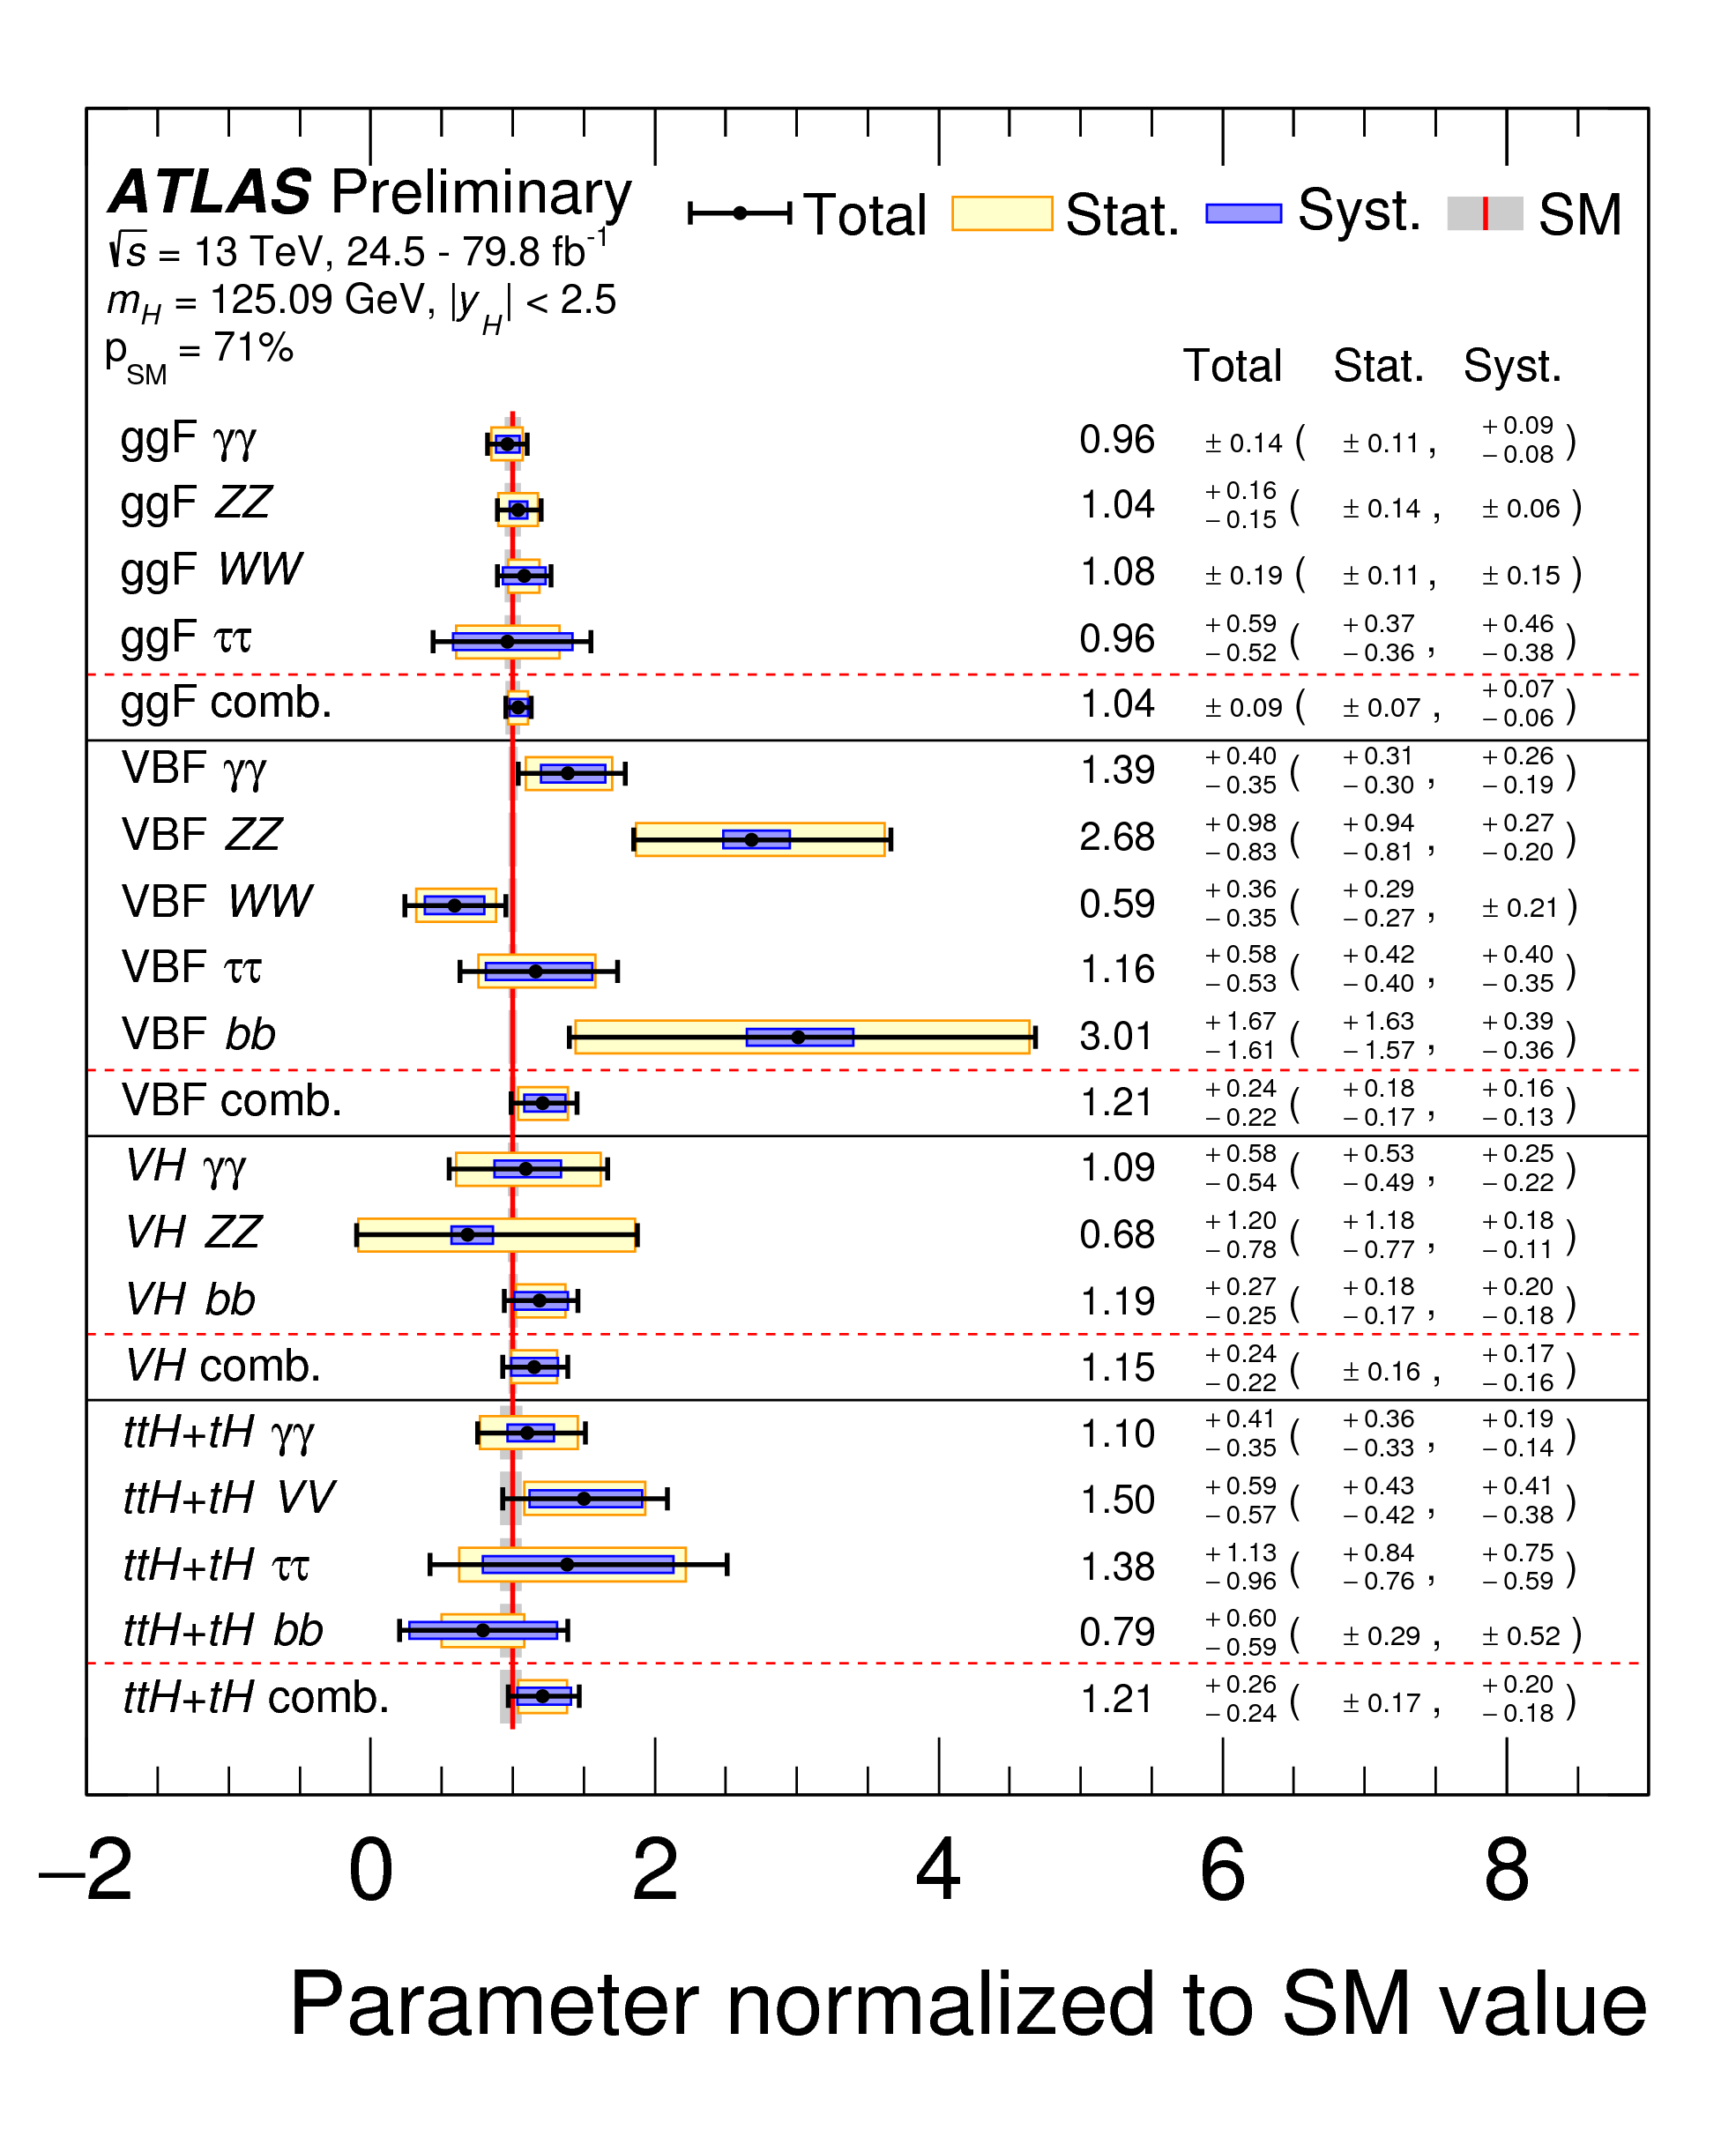
\includegraphics[width=4in]{figures/chapter6/higgs_comb_plot.png}
    \caption{Cross-sections times branching fractions for relevant Higgs production and decay modes normalized to the SM predicted values. The values are obtained by a simultaneous fit to all channels \cite{higgs_comb_paper}.}
    \label{fig:higgs_comb}
\end{figure}

Although ggF and VBF are the dominant Higgs production modes, VH is a particularly interesting channel for studying $H\rightarrow\tau\tau$ decays. Both $Z$ and $W^{\pm}$ bosons can decay to light leptons ($e$ and $\mu$) at branching ratios suitable for observation at the LHC: approximately 3\% for $Z\rightarrow e^+e^-$ and $Z\rightarrow\mu^+\mu^-$ and 10\% for $W^{\pm}\rightarrow e^{\pm}\nu$ and $W^{\pm}\rightarrow \mu^{\pm}\nu$ \cite{pdg}. This allows the $VH,H\rightarrow\tau\tau$ analysis to exploit the highly efficient electron and muon triggers and IDs. This results in relatively low background contributions and  an unbiased $H\rightarrow\tau\tau$ decay. Thus this analysis provides an excellent opportunity to increase the precision of the $H\rightarrow\tau\tau$ branching ratio measurement. The Run-1 version of this search did not find statistically significant evidence for these processes (see Section \ref{sec:run1}) but increased increased luminosity and analysis design improvements make this a promising search for the full Run-2 dataset.

%% SECTION: DEFINITIONS
\section{Definitions}
This analysis encompasses four final states, or subchannels, defined by the decay products of the vector boson and taus; they can hence be referred to as VH and WH (for the boson type) and lep-had or had-had for the tau decay products. The selection requirements for the four channels are detailed in Section \ref{sec:anal_cats}. The basic object requirements is shared between all the channels and each channel uses a variable related to the reconstructed Higgs mass as the final distribution to fit (Section \ref{sec:mass_recon}). The criteria for all relevant objects and the methods of mass estimation are described below. 

%%OBJECTS
\subsection{Object Criteria}
In most cases, the object requirements are chosen to be as close to the Run-1 criteria as possible \cite{vh_run1_note}. All requirements are selected from the recommendations supported by the relevant ATLAS Working Groups. Additionally, when possible, they are chosen to be compatible with the ggF/VBF $H\rightarrow\tau\tau$ Run-2 measurement. 

\subsubsection{Taus}
This analysis uses taus that are seeded by anti-$k_t$ R=0.4 jets and further reconstructed and identified as described in Chapter 3. All taus must have a minimum $p_T$ of 25 GeV and be exactly 1- or 3-pronged. 1-pronged taus must have clusters and a leading track with $|\eta|<2.47$ and 3-pronged taus must be withing $|\eta|<2.5$. Additionally, taus must pass the medium BDT-based operating point as defined by the Tau Working Group \cite{tau_cp}; this corresponds to an efficiency of approximately 55-60\%. The final analysis will likely incorporate the new RNN-based tau ID (Chapter 3).

\subsubsection{Muons}
Muons used in this analysis must be combined muons which are reconstructed and identified as described in Chapter 3. They must have a minimum $p_T$ of 3.5 GeV and be in the region $|\eta|<2.5$. They are required to pass the Loose operating point and track quality criteria as defined by the Muon Working Group \cite{muon_cp}. This corresponds to an efficiency of over 95\%.

\subsubsection{Electrons}
Electrons are reconstructed and identified as described in Chapter 5. They are required to be in the region $|\eta|<2.47$ and pass the Loose LH-based operating point and object quality criteria as set by the EGamma Working Group \cite{egam_cp}. They are additionally required to pass calorimeter cluster and track isolation requirements that the sum of transverse energy in the calorimeter (tracks) within a cone of size R=0.4 (R=0.2) around the electron cluster to be less than 8\% of the electron $E_T$. Collectively this provides an efficiency between 80 and 90\% depending on the $p_T$ and $|\eta|$ of the electron. Electrons in the  `crack' region of $1.37<|\eta|<1.52$ where the EM Calorimeter transitions from the barrel to endcap regions are required to pass the Medium LH-based operating point; these electrons are only used for overlap removal as described in Section \ref{sec:overlap} and not as analysis category objects due to decreased electron ID efficiency in the crack (see Chapter 5).\\

In order to exploit the lowered electron ID $p_T$ threshold for Run-2, the minimum electron $p_T$ for this analysis was lowered from 10 GeV (the Run-1 requirement) to 5 GeV. Preliminary studies, as shown in Figure \ref{fig:lowpt_cuflow}, indicate that this change allows additional events to pass the category requirements for the lep-had analysis channels. If further studies find that including these lower $p_T$ electrons does not substantially increase systematic uncertainties this would increase statistics in these channels.

\begin{figure}[htb!]
    \centering
    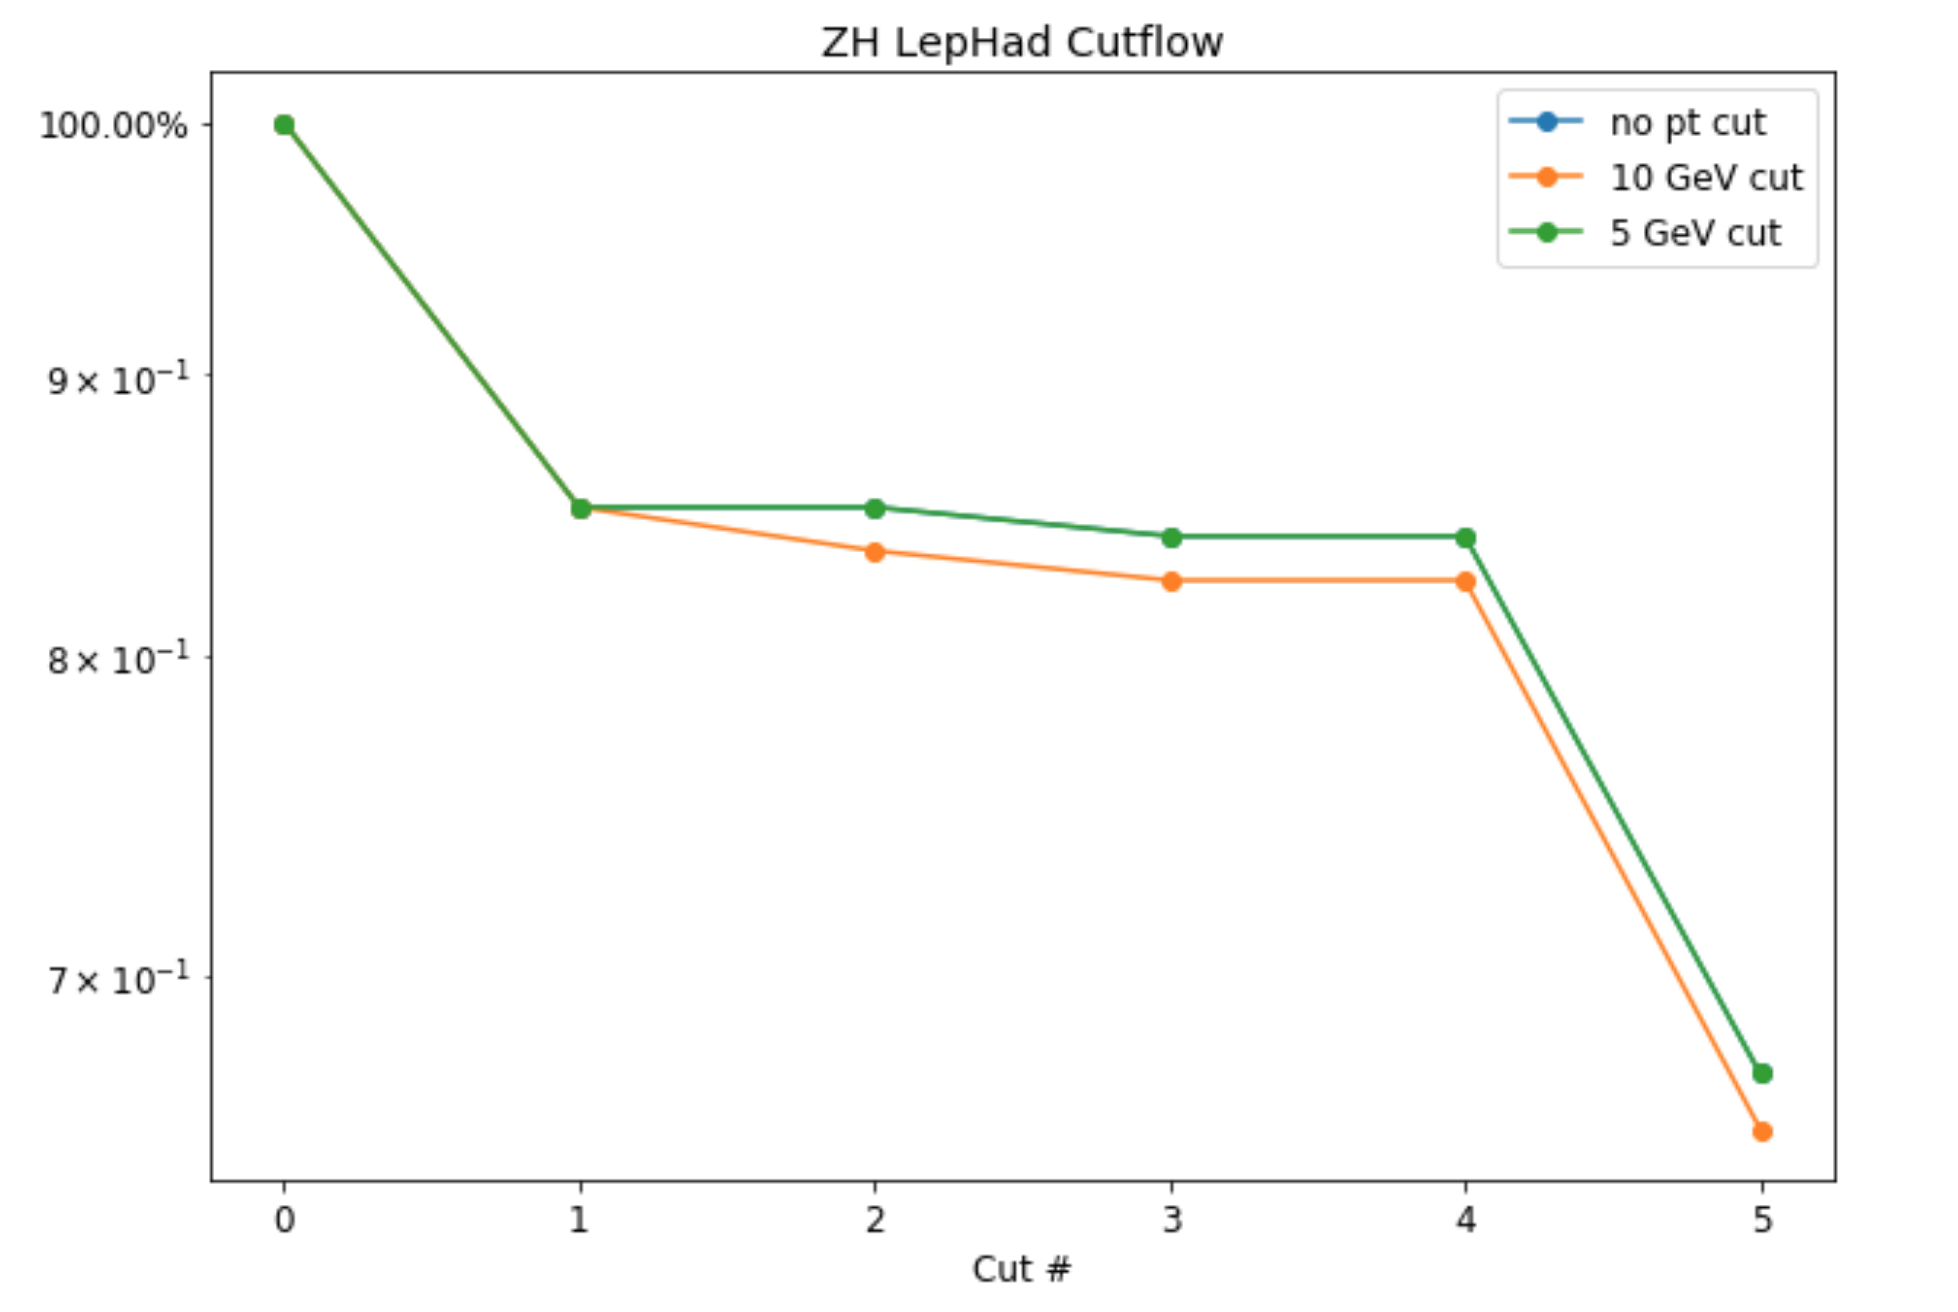
\includegraphics[width=4in]{figures/chapter6/lowpt_zhlephad_cutflow.png}
    \caption{Progressive cut flow for a portion of the ZH lep-had analysis category (after requiring exactly 3 leptons and one hadronic tau). Cut 2 is the $p_T$ cut of interest and other cuts are defined in Table \ref{tab:lowpt_cutflow}.}
    \label{fig:lowpt_cuflow}
\end{figure}

\begin{table}[htb!]
    \centering
    \begin{tabular}{|c|c|}
    \hline
    \textbf{Cut \#} & \textbf{Definition}\\
    \hline
    0 & All 3 leptons are tight\\
    1 & Two same flavor oppositely signed leptons with $80\text{GeV}<m_{ll}<100$GeV\\
    2 & Leptons pass min $p_T$ (10 GeV for the green curve and 5 GeV for the orange curve)\\
    3 & Tau passes BDT medium and is oppositely charged from 3rd lepton)\\
    4 & Tau $p_T<25$ GeV\\
    5 & 60GeV$<p_T(\text{tau + 3rd lepton})$\\
    \hline
    \end{tabular}
    \caption{Cut definitions for Figure \ref{fig:lowpt_cuflow}. See Section \ref{sec:zh_lephad} for additional details.}
    \label{tab:lowpt_cutflow}
\end{table}

\subsubsection{Jets}
Jets are not considered as analysis category objects but multiple control regions and the WH analysis channels include b-jet vetos; thus it is necessary to define analysis-wide jet requirements. This analysis uses anti-$k_t$ reconstructed jets (Chapter 3) with a maximum radius of R=0.4. Only jets with $p_T>$30 GeV and $|\eta|<2.5$ are used. Jet energies are callibrated according to the recommendations of the JetETMiss Working Group \cite{jet_met_cp}. A fixed-cut b-tagging requirement corresponding to an 85\% efficiency is used.

\subsubsection{MET}
Requirements on MET are not included in the four analysis category definitions but MET is used to separate the ZH and WH fake factor measurement regions (see Chapter 7) and as input to the mass estimation algorithms described in Section \ref{sec:mass_recon}. MET is calculated as described in Chapter 3 using calorimeter energy deposits associated to and calibrated according to the reconstructed objects outlined above. Additional energy deposits that are not associated to a physics object are scaled by a dedicated algorithm to improve resolution in high-pileup events.

%%OVERLAP
\subsection{Overlap Removal}\label{sec:overlap}
In some cases, certain tracks and calorimeter clusters may be reconstructed as multiple objects and thus it is necessary to define a prioritization order. In the case where objects which pass the requirements outlined above overlap within a $\Delta R$ of 0.2 only one of them is preserved for input to the analysis category definitions. The overlap is resolved in the following order: muons $>$ electrons $>$ taus $>$ jets. This procedure uses muons with a reduced minimum $p_T$ of 2 GeV and precedes the electron isolation requirement application.

%%MASS RECON
\subsection{Mass Reconstruction}
After estimating background contributions (Chapter 7) and accounting for systematic and statistical uncertainties, the final result in all four analysis channels is obtained from a fit of the estimated di-tau invariant mass spectrum; the signal distribution should correspond to the Higgs mass of 125 GeV. However, as all event categories contain one or more neutrinos in the final state, the mass distribution must be calculated in a way that accounts for the missing energy of the neutrinos. This is done separately for the ZH and WH categories using the methods described below.

%% mmc
\subsubsection{Missing Mass Calculator}\label{sec:mass_recon}
In the ZH analysis categories, neutrinos only come from the tau decays and there can be two (had-had case) or three (lep-had case) final state neutrinos. For these channels, the di-tau mass is reconstructed using the Missing Mass Calculator (MMC) \cite{mmc}. This method takes the $x$- and  and $y$-components of the event's missing $p_T$ and the visible mass of the tau pair as inputs. This system is inherently under-constrained because the individual orientation components of the multiple final state neutrinos are all unknown. To manage this, the MMC method implements a scan over all possible neutrino momentum values and the most likely di-tau mass is selected based on the fact that the probability of a given distance ($\Delta R$) between the visible and invisible decay products of a tau decay is known. A sample of the $\Delta R$ probability distributions used to develop the MMC likelihood are shown in Figure \ref{fig:mmc_probs} and an example of a Run 1 MMC distribution is shown in Figure \ref{fig:mmc_run1} where a clear separation between the $H\rightarrow \tau\tau$ mass and $Z\rightarrow\tau\tau$ mass is visible. 

\begin{figure}[htb!]
    \centering
    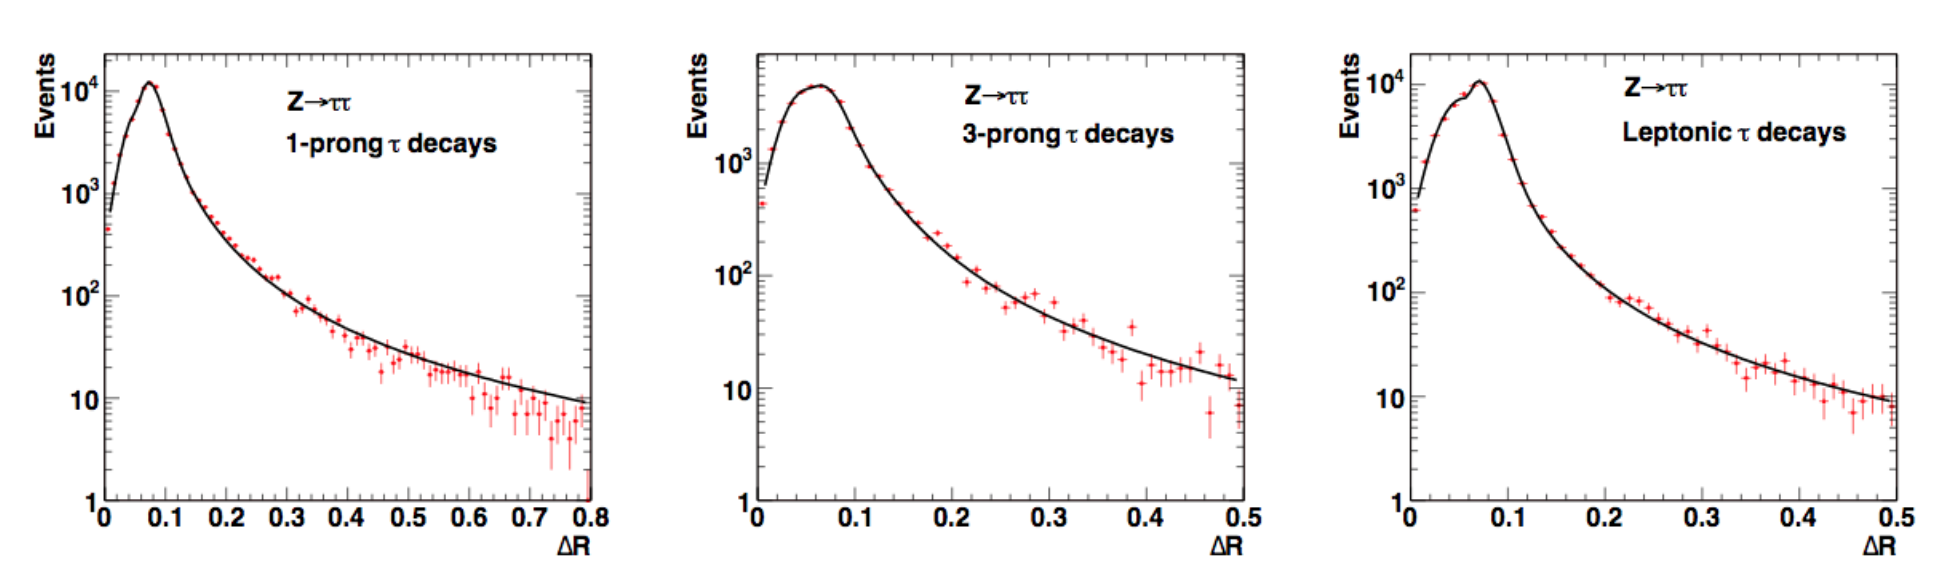
\includegraphics[width=5.5in]{figures/chapter6/mmc_probs.png}
    \caption{Examples of the probability distribution functions of $\Delta R$ for 1-prong hadronic tau decays (left), 3-prong hadronic tau decays (middle) and leptonic tau decays (right) \cite{mmc}.}
    \label{fig:mmc_probs}
\end{figure}

\begin{figure}[htb!]
    \centering
    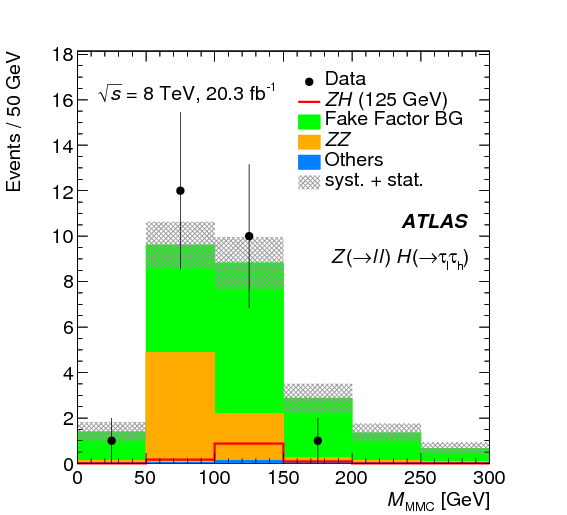
\includegraphics[width=3in]{figures/chapter6/mmc_run1.png}
    \caption{Run 1 MMC distribution after signal region cuts for the ZH lep-had channel. \cite{vh_run1_paper}.}
    \label{fig:mmc_run1}
\end{figure}

%% m2t
\subsubsection{Late Transverse Projected Mass}
In both the WH categories there is an additional neutrino from the W decay which makes the MMC method sub-optimal. Instead, the Late Projected Transverse Mass ($M_{2T}$) method is used as described in \cite{m2t}. This method calculates a lower bound for the di-tau combined mass in a given event by minimizing over the allowed phase-space of possible neutrino momentum. The resulting distribution is bounded above by the Higgs mass.\\

The final state objects in the event are partitioned first into groups based on their parent particle (W or H in this case) and then into visible and invisible categories (Figure \ref{fig:m2t_diag}). The transverse momentum projection of each partition is determined: $\Vec{\bf{p}}_{aT}=\sum_{i \in V_a}\Vec{p}_{iT}$ for the visible daughters of parent particle $a$ and $\Vec{\bf{q}}_{aT}=\sum_{i \in I_a}\Vec{q}_{iT}$ for the invisible daughters of parent particle $a$. The transverse energy projection of each partition can then be calculated: ${\bf{e}}_{aTv(i)}=$

\noindent $\sqrt{(\sum_{i \in V_a(I_a)}E_i)^2-(\sum_{i \in V_{a}(I_a)}p_{iz})^2}$ and the transverse energy-momentum vectors are determined: ${\bf{p}}^{\alpha}_{aT}=({\bf{e}}_{aTv},\Vec{\bf{p}}_{aT})$ for the visible components of particle $a$ and ${\bf{q}}^{\alpha}_{aT}=({\bf{e}}_{aTi},\Vec{\bf{q}}_{aT})$ for the invisible components of particle $a$. The late-projected transverse mass of particle $a$ is then $M_{aT}=\sqrt{g_{\alpha\beta}({\bf{p}}^{\alpha}_{aT}+{\bf{q}}^{\alpha}_{aT})({\bf{p}}^{\beta}_{aT}+{\bf{q}}^{\beta}_{aT})}$ where $g_{\alpha\beta}$ is the Minkowski metric. The $M_{2T}$ method then considers the largest parent mass ($\max_{a}[M_{aT}]$) and minimizes this value over all possible values of the invisible particles' (neutrinos') momenta. This defines the value 
$$M_{2T}=\min_{\sum\Vec{q}_{iT}=\Vec{p}_T^{miss}}(\max_{a}[M_{aT}]).
$$\\

\begin{figure}[htb!]
    \centering
    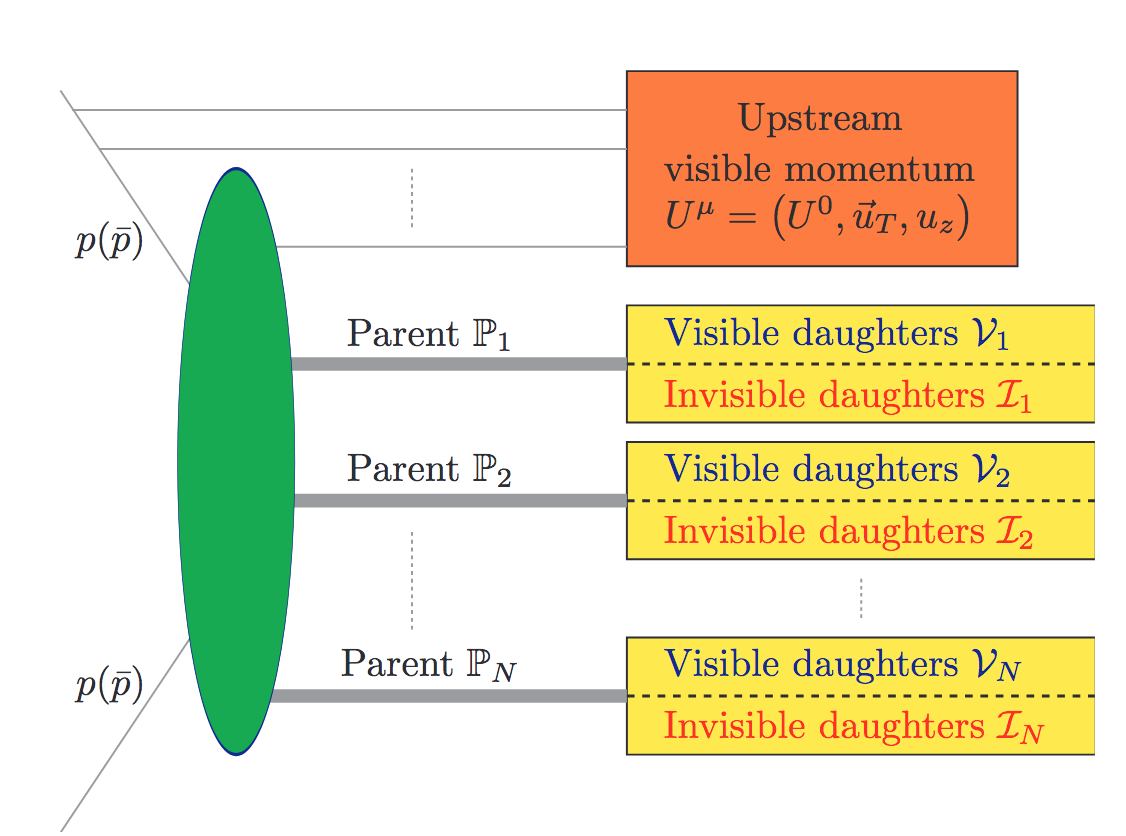
\includegraphics[width=4in]{figures/chapter6/m2t_diag.png}
    \caption{Depiction of particle partitioning in the $M_{2T}$ method \cite{m2t}.}
    \label{fig:m2t_diag}
\end{figure}

The possible values over which $M_{2T}$ is maximized are constrained by requiring that the sum of the neutrino $p_T$ is equal to the MET of the event and invariant mass of the lepton and the neutrino attributed to the W be as close as possible to the W mass of 80.4 GeV. As defined, this phase-space is 9 dimensional in the had-had case (3 neutrinos with 3 momentum components) and 12 dimensional in the lep-had case. In order to reduce the phase-space, the neutrino momentum is approximated to be collinear with the visible tau decay products as $\Vec{p}_v=(\frac{1}{x}-1)\Vec{p}_{vis}$ where $x=\frac{p_{vis}}{p_{vis}+p_v}$ is the fraction of the total tau momentum attributed to the visible decay products. The phase-space then becomes one-dimensional ($x$) for both the lep-had and had-had cases. An example of Run 1 $M_{2T}$ distributions is shown in Figure \ref{fig:m2t_plots}.

\begin{figure}[htb!]
    \centering
    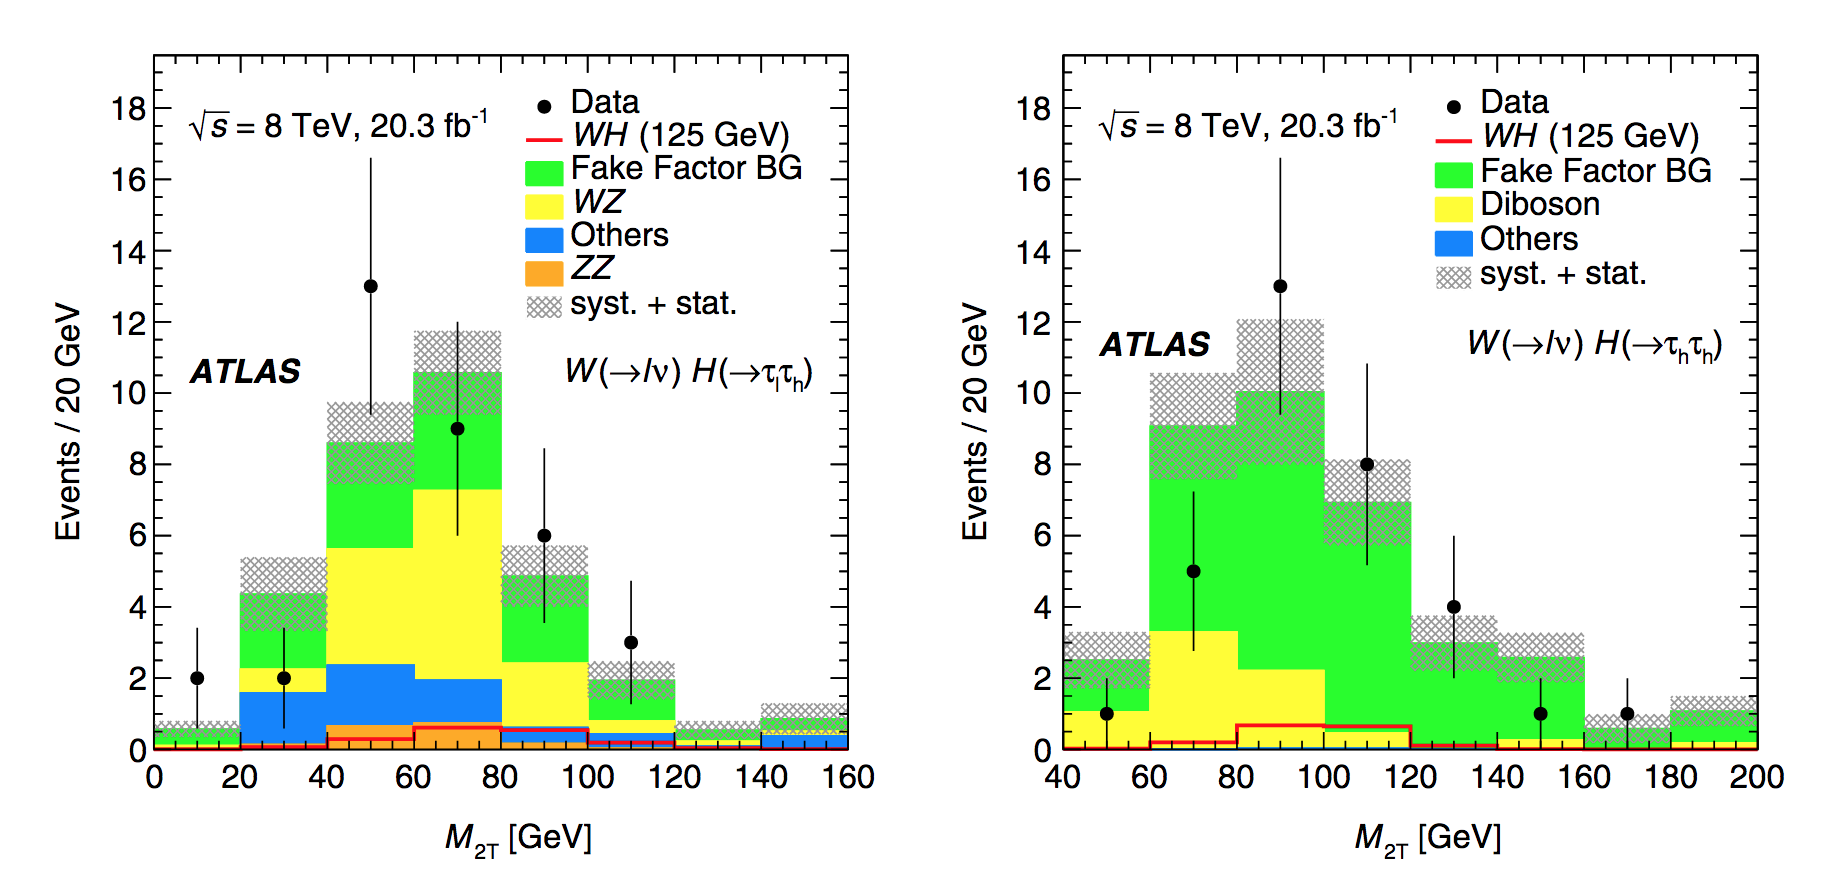
\includegraphics[width=5in]{figures/chapter6/m2t_plots.png}
    \caption{Run 1 $M_{2T}$ distributions for three Higgs mass values after signal region cuts for the WH lep-had channel (left) and WH had-had channel (right) \cite{vh_run1_paper}.}
    \label{fig:m2t_plots}
\end{figure}

%% SECTION: ANALYSIS CATEGORIES
\section{Analysis Categories}\label{sec:anal_cats}
This analysis is divided into four separate categories each with its own event selection criteria; the categories are defined by the type of vector boson produced in association with the Higgs (Z or W) and the decay modes of the taus (one leptonic and one hadronic or both hadronic). Each set of category requirements was developed to provide highly efficient background rejection while maintaining as many signal events as possible. In Run 1, this corresponded to an acceptance of 1.9\% for the WH channels and 5.3\% for the ZH channels. Any contributions from other Higgs processes after category selection was applied was found to be negligible \cite{vh_run1_paper}. \\

The common single-lepton and di-lepton triggers used so select events are shown in Table \ref{tab:triggers}. The $p_T$ of trigger objects used in the analysis is required to be 2 GeV above the trigger threshold in order to ensure maximal trigger efficiency.\\

\begin{table}[htb!]
\centering
   \begin{tabular}{r|c|c} % Column formatting, @{} suppresses leading/trailing space
      \hline
      Trigger & Trigger Threshold & Offline Threshold\\
      \hline
\verb!HLT_2mu14! & 14 GeV & 16 GeV \\
\verb!HLT_mu26_ivarmedium! & 26 GeV & 28 GeV \\
\verb!HLT_2e17_lhvloose_nod0! & 17 GeV & 19 GeV \\ 
\verb!HLT_e26_lhtight_nod0_ivarloose!& 26 GeV & 28 GeV \\
      \hline
   \end{tabular}
   \caption{Run 2 triggers used in the four analysis channels along with corresponding trigger and offline $p_T$ thresholds.}
   \label{tab:triggers}
\end{table}

The event selection requirements for each of the four categories are provided in the following sections. There are a number of control regions associated with each channel which are primarily used to validate the fake factor method described in Chapter 7. These control regions are described thoroughly in \cite{vh_run1_paper}.

%%WH LEPHAD
\subsection{$WH, \tau_{lep}\tau_{had}$}\label{sec:zh_lephad}
The WH channels are designed to select events where a Higgs boson is produced in association with a $W^{\pm}$ and the $W$ then decays to a lepton and a light neutrino (Figure \ref{fig:wh_feyn}). In the WH lep-had channel, the Higgs decays to two taus, one of which decays hadronically while the other decays leptonically.\\

\begin{figure}[htb!]
    \centering
    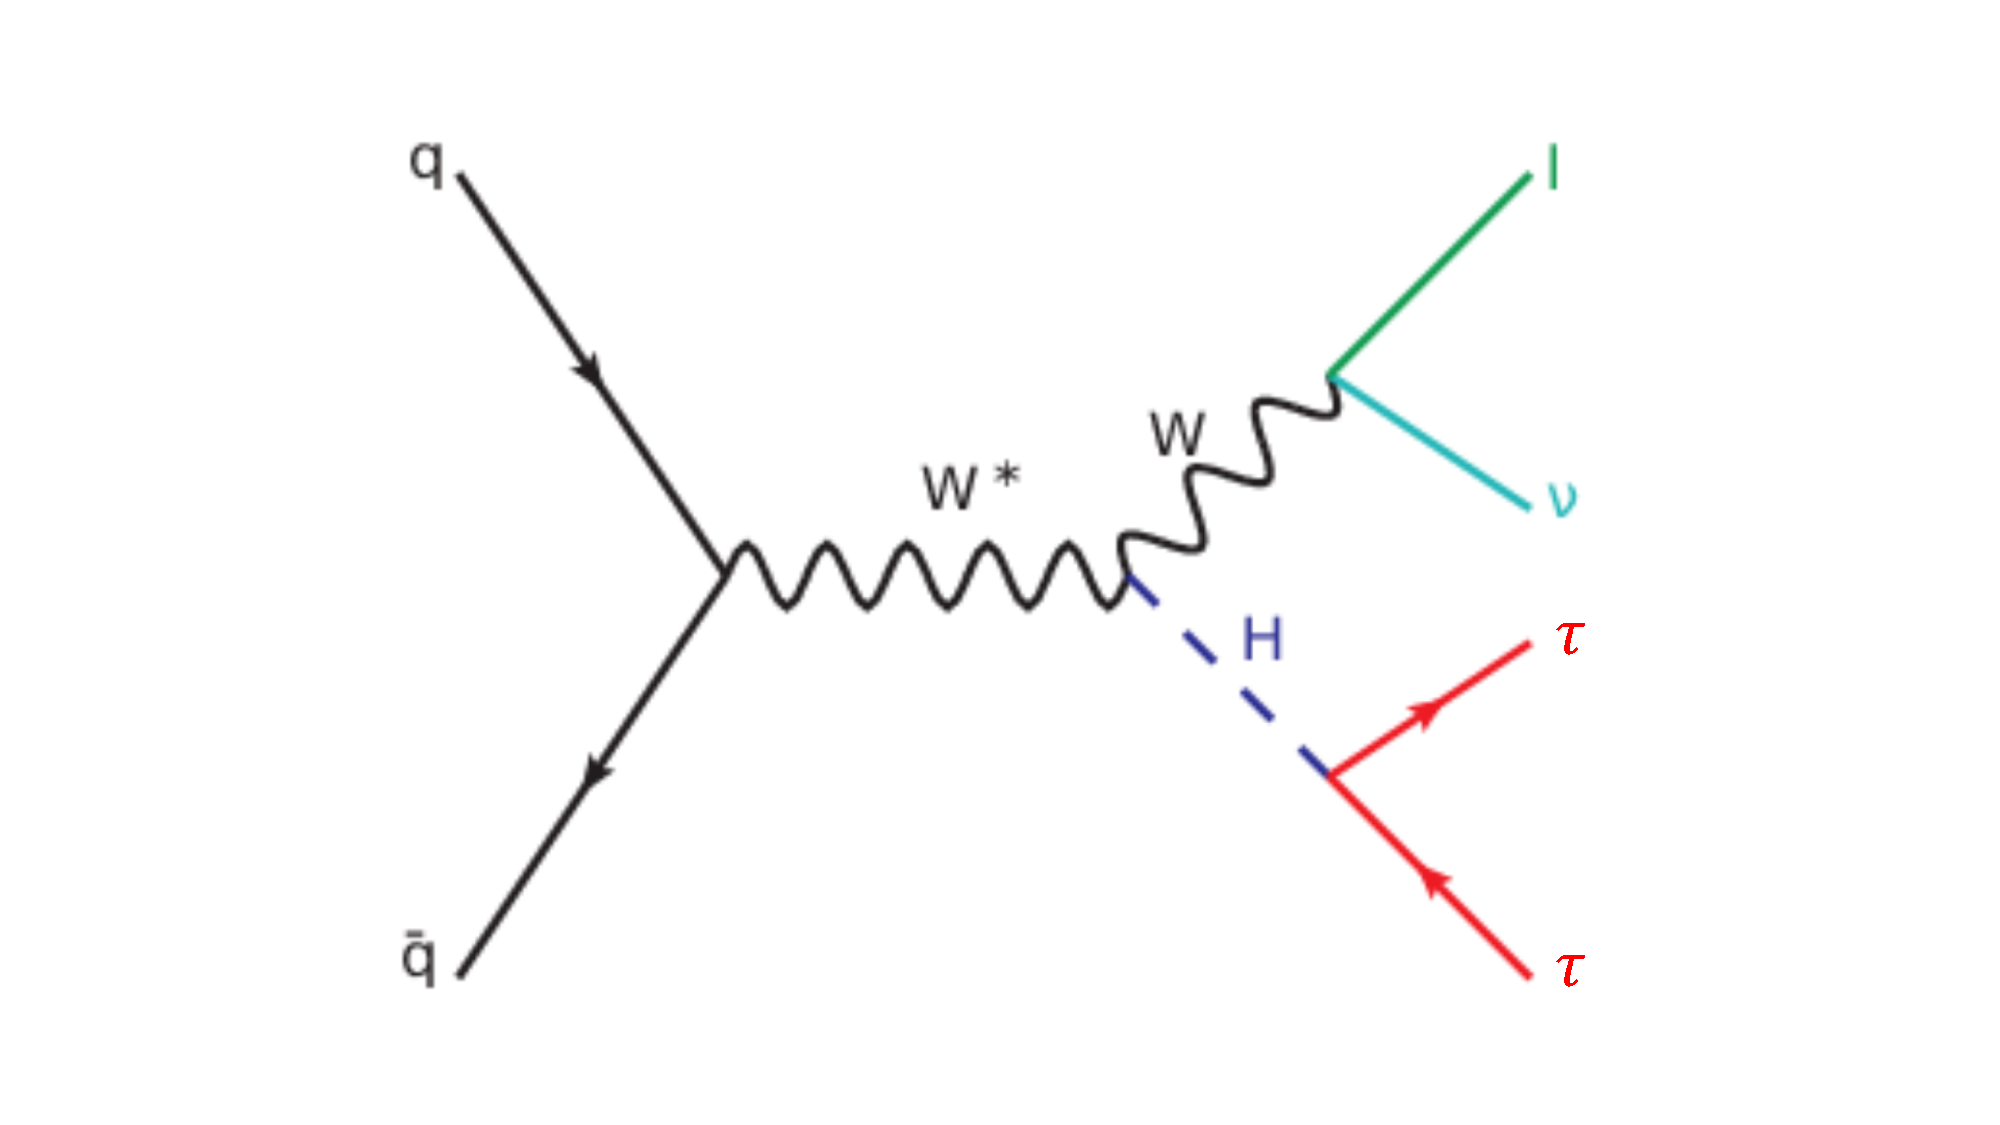
\includegraphics[width=2.5in]{figures/chapter6/wh_feynman.pdf}
    \caption{Feynman diagram for the leading order quark-initiated WH production.}
    \label{fig:wh_feyn}
\end{figure}

This analysis category requires exactly two opposite-flavor, tightly identified light leptons and one BDT-Medium tau. The light lepton with lowest $p_T$ is associated to the Higgs and the two light leptons are required to have the same charge to reduce backgrounds from $Z/\gamma*\rightarrow\tau\tau+jets$ events and $WW$ events where both Ws decay leptonically. The leptons must also both be isolated. A b-jet veto is applied to reduce background from $t\bar{t}$ events. The tau is required to have opposite charge from the two light leptons and the total $p_T$ of the three leptons must be greater than 80 GeV. This $p_T$ requirement significantly reduces the Z+jets and multijets backgrounds which come mainly from low $p_T$ jets mis-identified as taus. An additional requirement that $\Delta R(\tau_{lep}\tau_{had})<3.2$ further lowers these backgrounds. 

%%WH HADHAD
\subsection{$WH, \tau_{had}\tau_{had}$}
The WH had-had category requires both Higgs associated taus to decay hadronically. In this case, the highest $p_T$ lepton in the event is associated to the W. Events are first selected by requiring exactly two oppositely charged BDT-Medium taus and one tight, isolated light lepton. A b-jet veto is applied to reduce backgrounds from $t\bar{t}$ events. Events are required to have a combined transverse mass between the lepton and MET of at least 20 GeV to reject $Z\rightarrow\tau\tau$ background. The two taus are required to be separated by $0.8<\Delta R<2.8$ in order to reduce contributions from di-jet backgrounds. Finally, the scalar sum of the $p_T$ of the three leptons must be at least 100 GeV to reduce the background from multi-jet events.

%%ZH LEPHAD
\subsection{$ZH, \tau_{lep}\tau_{had}$}
The ZH channels are designed to select events where a Higgs boson is produced in association with a Z boson and the Z then decays to a same-flavor opposite charge pair of light leptons (Figure \ref{fig:zh_feyn}). In the ZH lep-had channel, the Higgs decays to two taus, one of which decays hadronically while the other decays leptonically.\\

\begin{figure}[htb!]
    \centering
    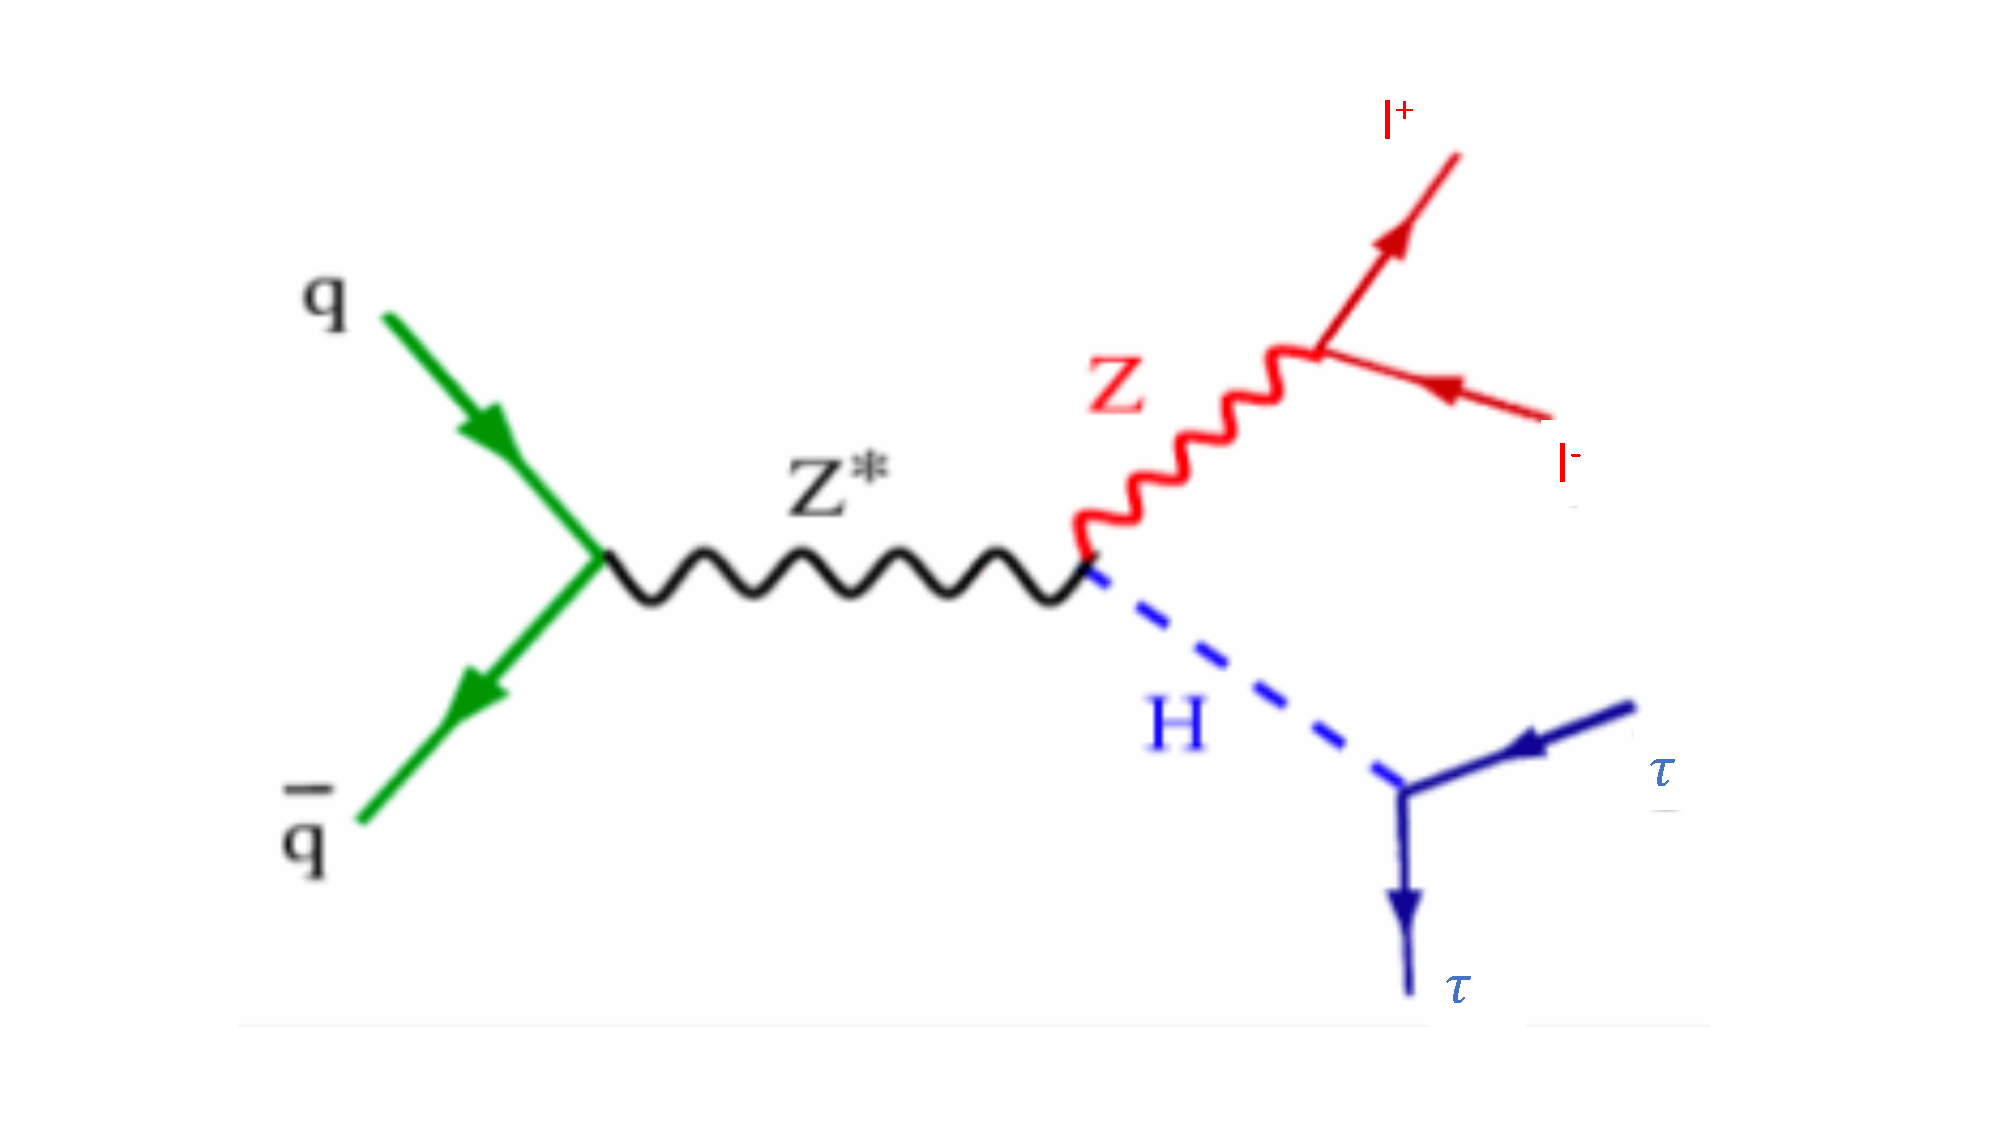
\includegraphics[width=2.5in]{figures/chapter6/zh_feynman.pdf}
    \caption{Feynman diagram for the leading order quark-initiated ZH production. There are also contributions from gluon initiated triangle and box diagrams.}
    \label{fig:zh_feyn}
\end{figure}

Events in this category are required to have exactly three light leptons and one BDT-Medium tau. The two same-flavor opposite-charge leptons with invariant mass closest to 91 GeV are associated to the Z and this mass must be between 80 and 100 GeV. The remaining lepton and the tau are associated to the Higgs and are required to have opposite charge. They must have a combined scalar $p_T$ sum of at least 60 GeV to suppress Z+jets backgrounds.  

%% ZH HADHAD
\subsection{$ZH,\tau_{had}\tau_{had}$}
The ZH had-had category requires both Higgs-associated taus to decay hadronically. These events are required to have exactly two same-flavor opposite-charge light leptons and two BDT-Medium taus. The invariant mass of the two light leptons must be between 60 and 120 GeV. The two taus must be opposite change and have a scalar $p_T$ sum of at least 88 GeV to reduce Z+jets backgrounds. 

%% SECTION: RUN 1
\section{Run-1 Results}\label{sec:run1}
In Run-1, the final observed signal strength $\mu$ of this analysis was determined using a binned global maximum-likelihood fit as described in \cite{lh_fit_method_paper} to the Higgs candidate mass spectra. As described in Section \ref{sec:mass_recon}, the MMC distribution was fit for both ZH channels and the $M_{2T}$ distribution was fit for both WH channels. A set of nuissance parameters $\Vec{\theta}$ was used in the fit to account for systematic uncertainties and the expected number of signal and background events in each mass distribution bin was calculated as a function of these parameters. The test statistic $q_{\mu}$ was constructed as a function of the profile likelihood ratio and this statistic was used to measure the compatibility of the binned data with the background-only hypothesis and to set Confidence Level (CL) intervals on the final result. Finally, a significance was calculated to quantify the probability of obtaining the observed values of $q_{\mu}$ if the true signal strength was $\mu=1$. Generally a significance of at least 3$\sigma$ is required to qualify a process for observation and 5$\sigma$ is required to qualify for discovery.\\

The results of the Run 1 analysis can be seen in Figures \ref{fig:conf_int} and \ref{fig:sig_stren}. The measured signal strength for a 125 GeV Higgs, normalized to the SM expectation, was $\mu=2.3\pm1.6$. The combined 95\% confidence interval on the ratio of the observed cross-section to the SM predicted cross-section was 5.6. This was above the expected value for both the signal included and background-only hypotheses, but was nonetheless consistent with the expected values within uncertainty. A major challenge of the Run-1 analysis was low statistics in all analysis channels; this allowed slight data excesses in both had-had channels to substantially weaken the cross-section measurement limit. Finally, the expected and observed significance for each analysis channel is shown in Table \ref{tab:run1_sig}.\\

\begin{figure}[htb!]
    \centering
    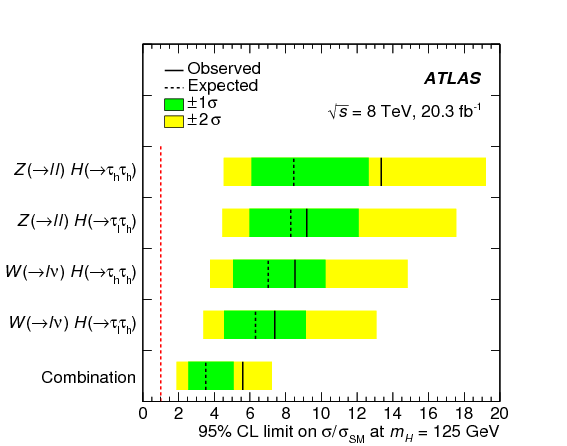
\includegraphics[width=3.2in]{figures/chapter6/conf_intervals_run1.png}
    \caption{The Run-1 95\% CIs on the ratio of measured cross-section to SM cross-section for each channel individually and all four combined \cite{vh_run1_paper}.}
    \label{fig:conf_int}
\end{figure}

\begin{figure}[htb!]
    \centering
    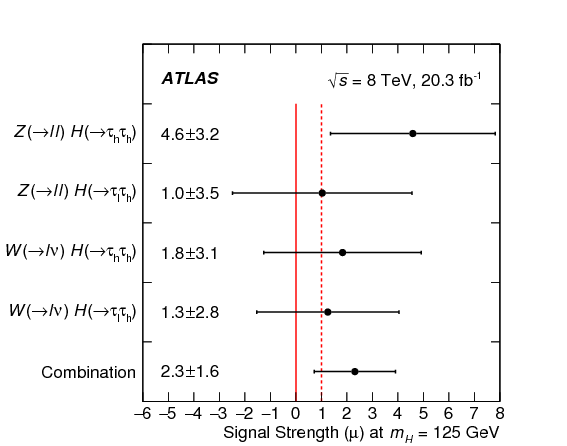
\includegraphics[width=3.2in]{figures/chapter6/sig_strength_run1.png}
    \caption{The Run-1 signal strength $\mu$ for each analysis channel individually and all four combined \cite{vh_run1_paper}.}
    \label{fig:sig_stren}
\end{figure}

\begin{table}[htb!]
    \centering
    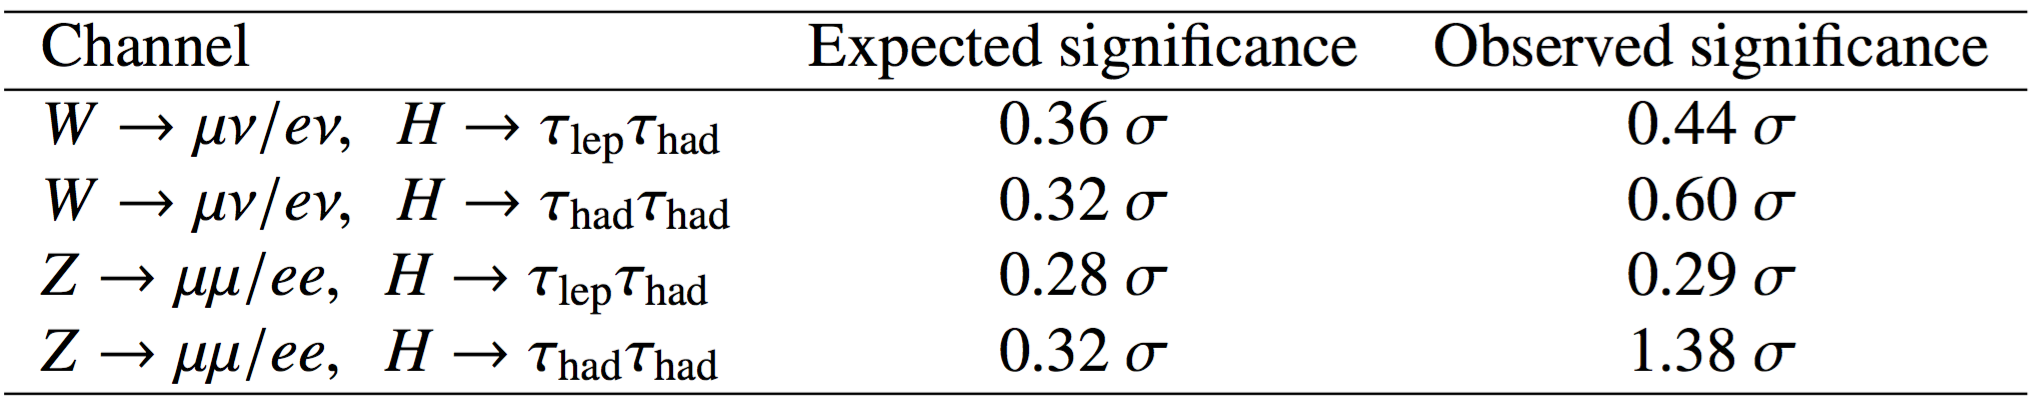
\includegraphics[width=4in]{figures/chapter6/run1_sig.png}
    \caption{The Run-1 expected and observed significance for each of the four analysis channels \cite{vh_run1_paper}.}
    \label{tab:run1_sig}
\end{table}

The current status of the Run 2 analysis and planned improvements are described in Chapters 7 and 8.